\documentclass{beamer}
\usetheme{Frankfurt}
\setbeamertemplate{footline}[frame number]
\setbeamercovered{transparent}
\usepackage{graphicx,animate,tikz,amsmath}
\graphicspath{{../images/}}


\AtBeginSection[]{
	\begin{frame}
	\vfill
	\centering
	\begin{beamercolorbox}[sep=8pt,center,shadow=true,rounded=true]{title}
		\usebeamerfont{title}\insertsectionhead\par%
	\end{beamercolorbox}
	\vfill
\end{frame}
}

\title{SPH simulations for space defense}
\author{Maximilian Rutz}

\begin{document}
	
\begin{frame}[plain]
    \maketitle
\end{frame}

\begin{frame}[plain]{Roadmap}
\tableofcontents
\end{frame}

\section{Dart and Hera missions}
\begin{frame}
	\begin{tikzpicture}[remember picture,overlay]
		\node[at=(current page.center)] {
		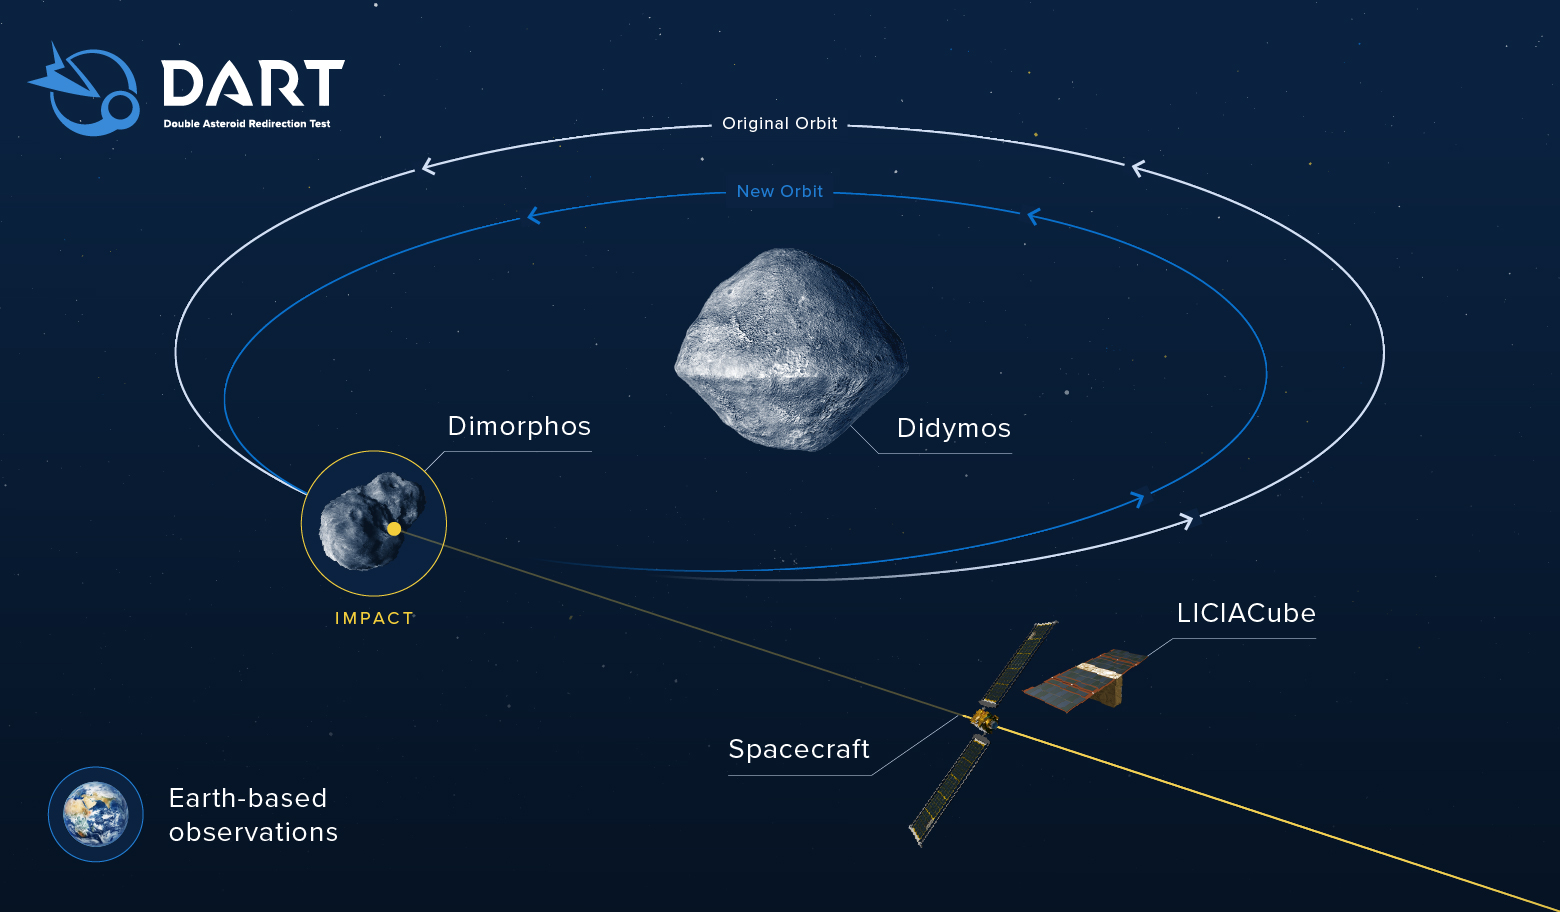
\includegraphics[keepaspectratio,
		width=\paperwidth,
		height=\paperheight]{dart_mission.jpg}};
	\end{tikzpicture}
\end{frame}

\begin{frame}{Dart Mission}
	%https://dart.jhuapl.edu/Gallery/media/graphics/lg/DART-infographic_v4.jpg
	\begin{itemize}
		\item Launch in July 2021 on a SpaceX Falcon 9 \pause
		\item Impact in fall 2022 \pause
		\item Impact at ~0.04 au to Earth, ~15x Earth-Moon, ~1/10x Earth-Mars \pause
		\item Observations with LICIACube and earth based telescopes
	\end{itemize}
\end{frame}

\begin{frame}{Hera Mission}
	\begin{tikzpicture}[remember picture,overlay]
	\node[at=(current page.center)] {
		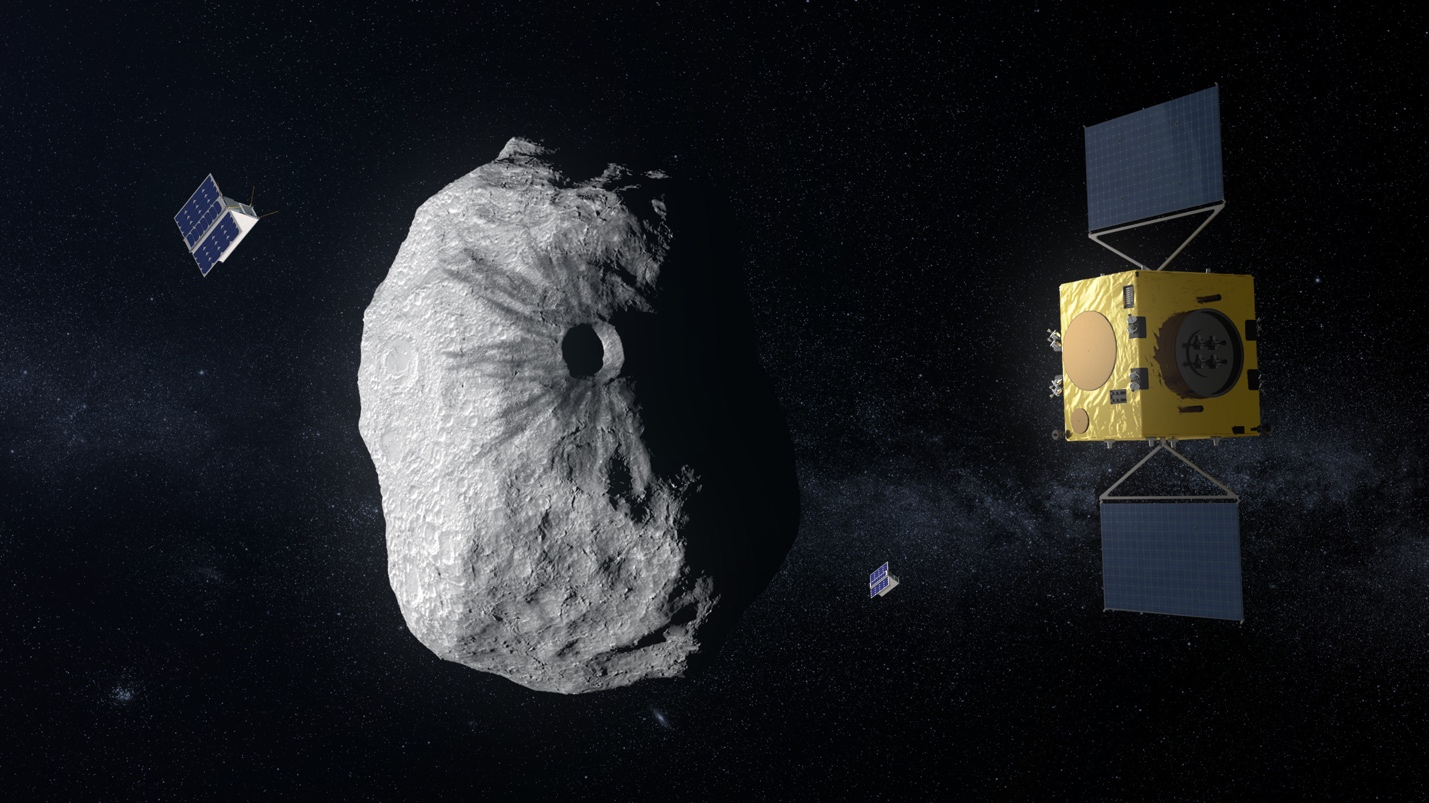
\includegraphics[keepaspectratio,
		width=\paperwidth,
		height=\paperheight]{hera_mission.jpg}};
	\end{tikzpicture}
\end{frame}

\begin{frame}{Hera Mission}
%https://www.esa.int/var/esa/storage/images/esa_multimedia/images/2018/06/testing_deflection/1%5359917-7-eng-GB/Testing_deflection_pillars.jpg
	\begin{itemize}
		\item Launch in 2024 \pause
		\item Arrival in 2026 \pause
		\item Why a second mission? \pause
		\begin{itemize}
			\item Dust cloud after impact \pause
			\item Reduce uncertainty of orbital shift \pause
			\item Politics \pause
		\end{itemize}
	\end{itemize}	
\end{frame}

\begin{frame}
	\begin{tikzpicture}[remember picture,overlay]
		\node[at=(current page.center)] {
		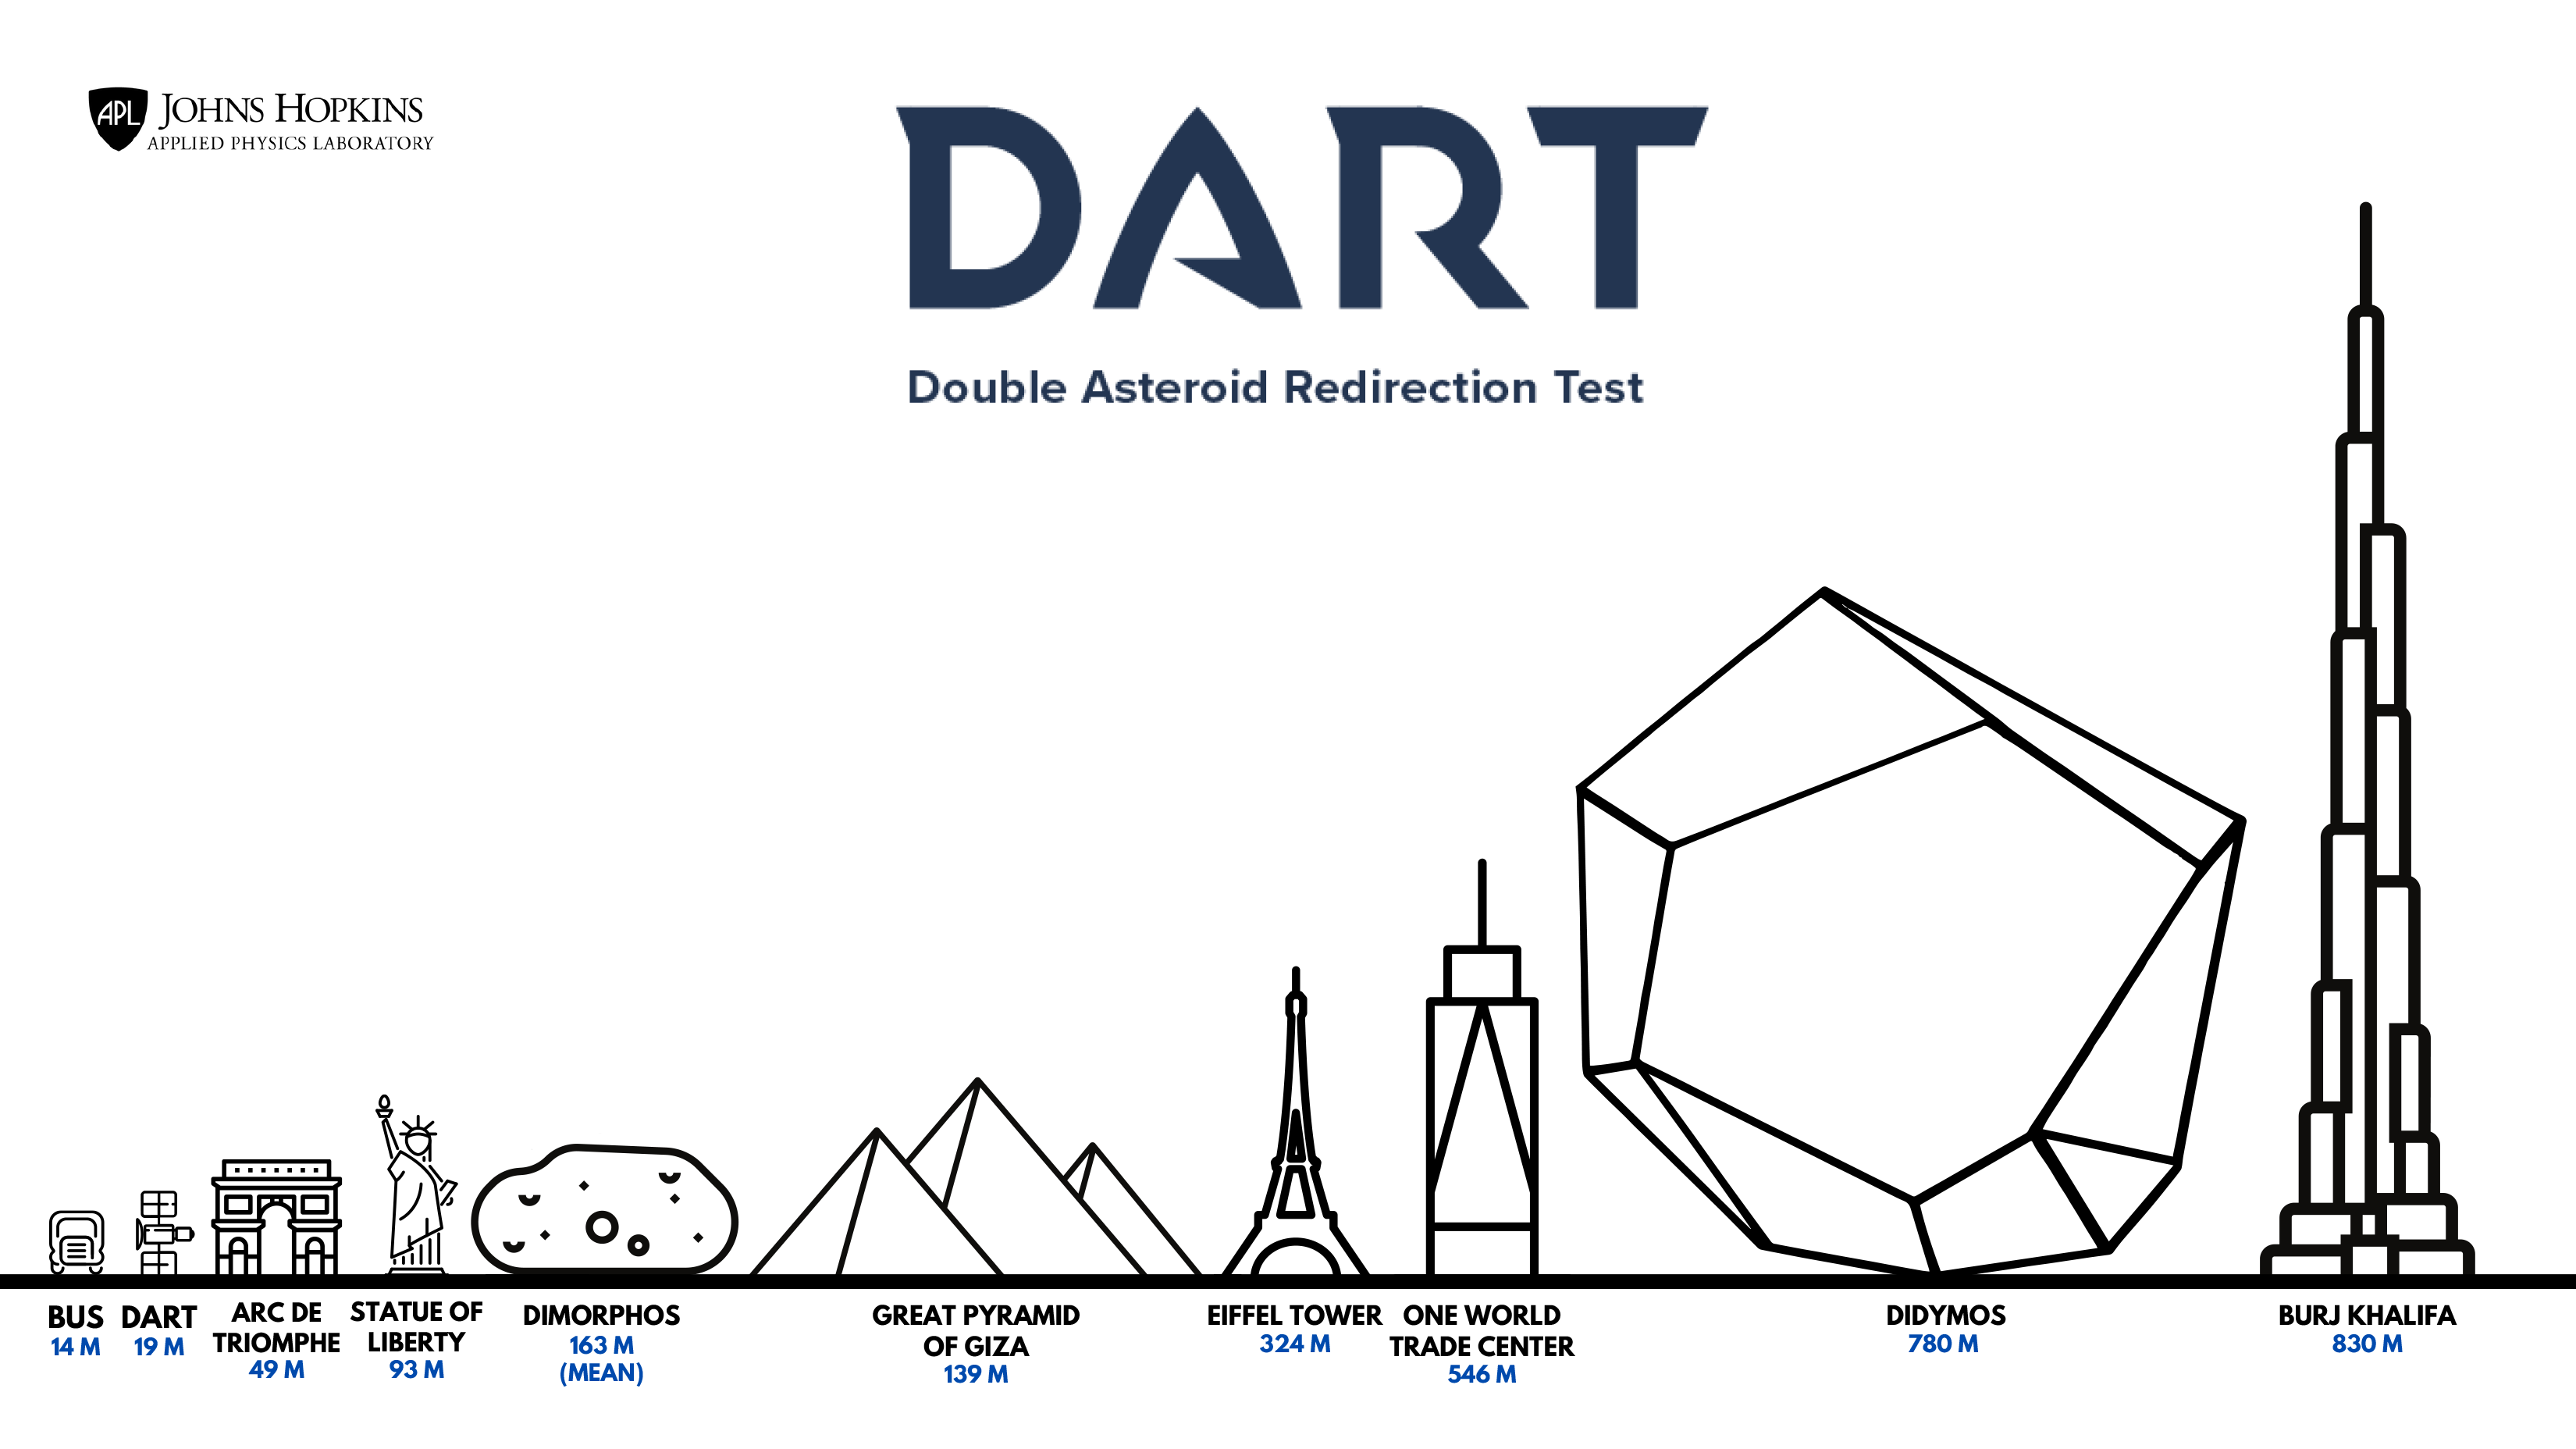
\includegraphics[keepaspectratio,
		width=\paperwidth,
		height=\paperheight]{asteroids_size.png}};
	\end{tikzpicture}
\end{frame}	

\section{SPH setup}
\begin{frame}{Simulation goals}
Compare numerical results with observations to:
\begin{enumerate}
	\item test numerical codes \pause
	\item identify target properties through parameter studies
\end{enumerate}
\end{frame}

\begin{frame}{Smoothed Particle Hydrodynamics}
	\begin{columns}
		\begin{column}{0.55\textwidth}
			\begin{itemize}
				\item gridfree method
				\item particles move through space with a velocity
				\item particles carry physical quantities like density, pressure or energy
				\item hydrodynamic/continuum mechanics equations can be solved for every particle
				\item spatial resolution 
			\end{itemize}
		\end{column}
		\begin{column}{0.4\textwidth}
			\vspace{\topsep}	
			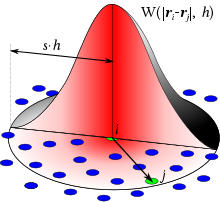
\includegraphics[width=\columnwidth]{sph_method.png}
		\end{column}
	\end{columns}
\end{frame}

\begin{frame}{Simulation scenario}
Target:
\begin{itemize}
	\item 160 meter diameter \pause
	\item important parameters such as porosity and strength unknown \pause
\end{itemize} 
Impactor:
\begin{itemize}
	\item 500 kg mass \pause
	\item 6 km/s impact velocity \pause
	\item main body 1.3 x 1.2 x 1.2 meter \pause
\end{itemize} 
\end{frame}


\begin{frame}{Miluphcuda solid models}
	\begin{itemize}
		\item fragmentation for brittle materials \pause
		\item p-$\alpha$ porosity model \pause
		\item shear strength \pause
		\item no self gravity \pause

	\end{itemize}
\end{frame}

\begin{frame}{Initial conditions}
	IMAGE 1st frame
\end{frame}

\begin{frame}{Initial conditions}
Target:
\begin{itemize}
	\item basalt \pause
	\item 20 meter diameter halfsphere \pause
	\item constant smoothing length in center \pause
\end{itemize} 
Impactor:
\begin{itemize}
	\item aluminum \pause
	\item 0.75 meter diameter sphere \pause
	\item 6 km/s impact velocity \pause
	\item 500 kg mass \pause
	\item same smoothing length as center of target \pause
\end{itemize} 
\end{frame}

\section{SPH results}
\begin{frame}{Beta factor}
Momentum change because of ejecta: $\boldsymbol{\beta} = 1 + \frac{p_{ejecta}}{p_{impactor}}$
Particles considered ejecta:
begin{itemize}
	\item positive velocity in opposite impact direction \pause
	\item above  \pause

\end{itemize} 
\end{frame}

%\begin{frame}{Target porosity and strength}
%	%\animategraphics[loop,controls,width=0.8\linewidth]{100}{bina%c}{0000}{0300}
%	exemplary video
%\end{frame}

\begin{frame}{Beta factor results}
	\begin{tikzpicture}[remember picture,overlay]
	\node[at=(current page.center)] {
		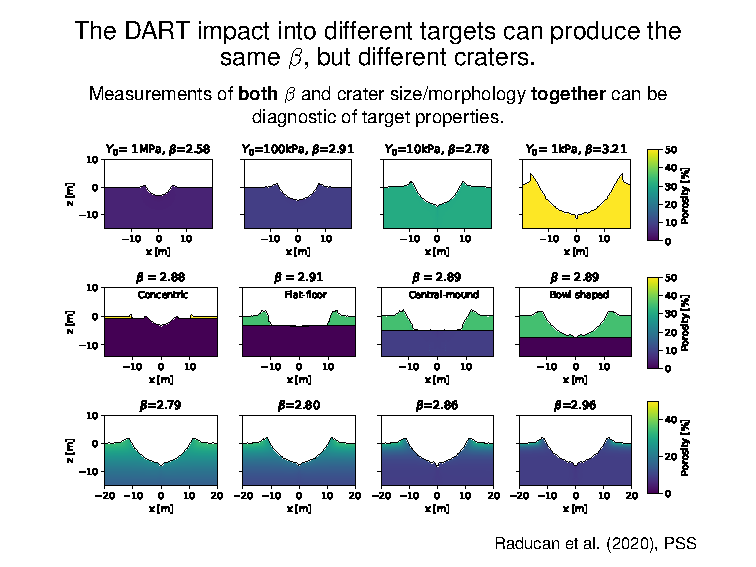
\includegraphics[keepaspectratio,
		width=\paperwidth,
		height=\paperheight]{cratering_raducan.pdf}};
	\end{tikzpicture}
\end{frame}

\begin{frame}{Beta factor other literature Stickle}
	\begin{tikzpicture}[remember picture,overlay]
	\node[xshift=0cm,yshift=2.5cm] at (current page.south) {
		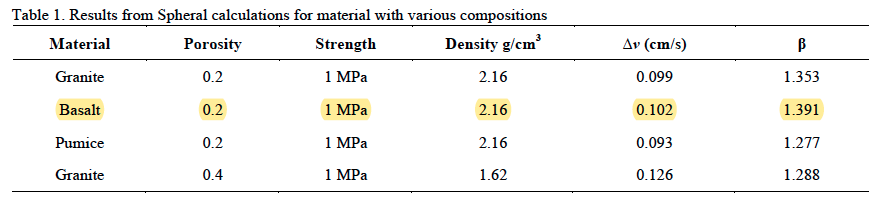
\includegraphics[keepaspectratio,
		width=\paperwidth,
		height=0.5\paperheight]{beta_stickle.png}};
	\end{tikzpicture}
\end{frame}

\begin{frame}{Beta factor other literature Raducan}
	\begin{tikzpicture}[remember picture,overlay]
	\node[xshift=0cm,yshift=2.5cm] at (current page.south) {
		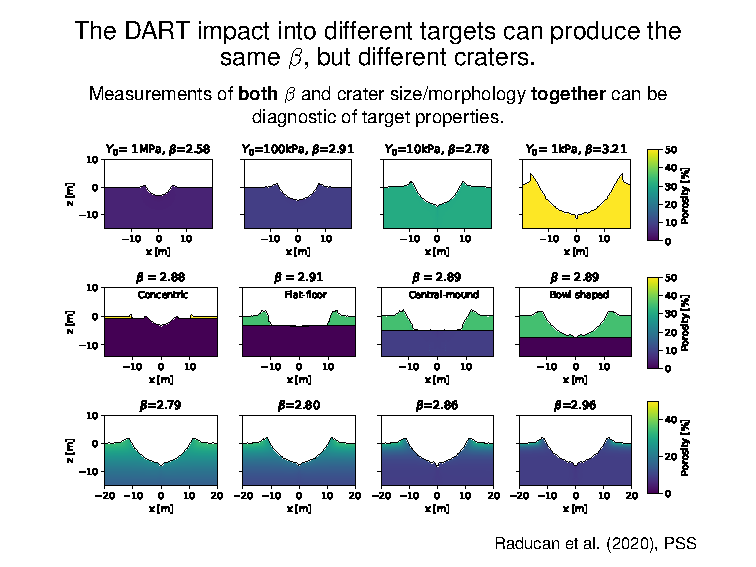
\includegraphics[keepaspectratio,
		width=\paperwidth,
		height=\paperheight]{cratering_raducan.pdf}};
	\end{tikzpicture}
\end{frame}

\begin{frame}{Crater shape}
	\begin{tikzpicture}[remember picture,overlay]
	\node[at=(current page.center)] {
	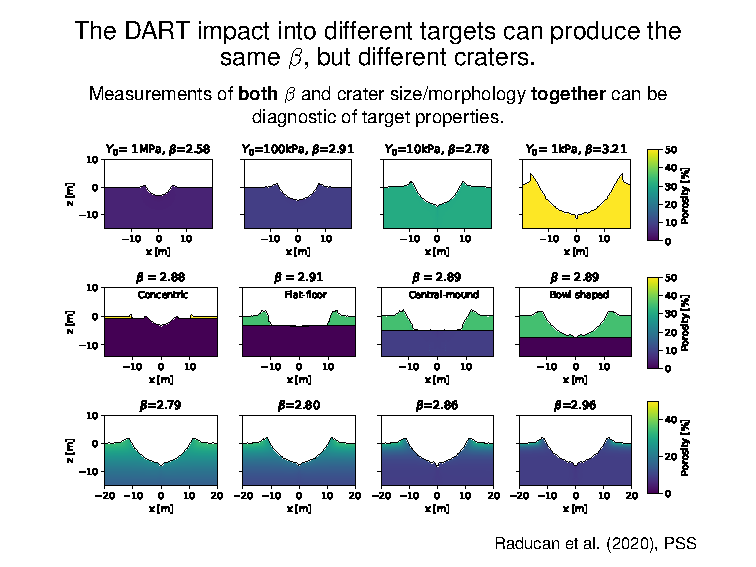
\includegraphics[keepaspectratio,
	width=\paperwidth,
	height=\paperheight]{cratering_raducan.pdf}};
\end{tikzpicture}
\end{frame}

\begin{frame}{Crater shape other literature}
	\begin{tikzpicture}[remember picture,overlay]
	\node[at=(current page.center)] {
		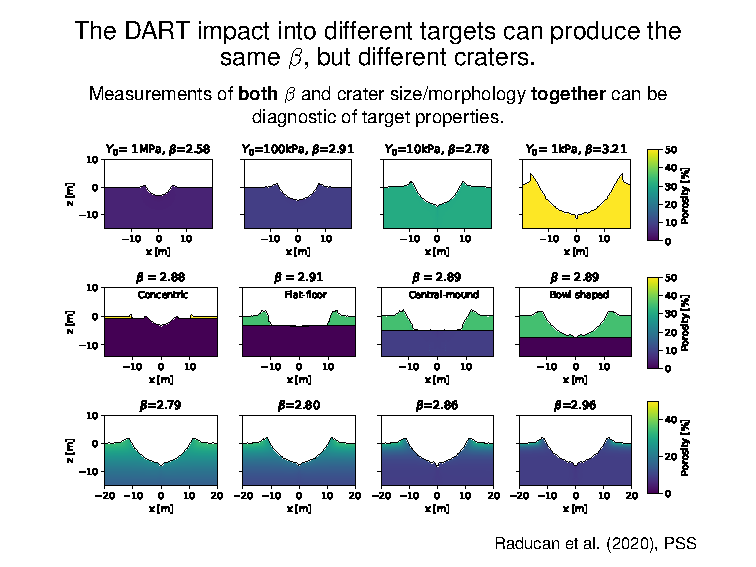
\includegraphics[keepaspectratio,
		width=\paperwidth,
		height=\paperheight]{cratering_raducan.pdf}};
	\end{tikzpicture}
\end{frame}

\begin{frame}{Personal observations about SPH}
	\begin{itemize}
	\item A lot of individual physics implementable 
	\item interaction between physical models within a code can get complex
	\item Many different codes available 
	\item Difficult to reproduce and compare results between different codes
	\item Dart setup could be useful as benchmark for solid models
	\end{itemize}
\end{frame}

\begin{frame}{Sources and additional information}
	Illustrations taken from Dart and Hera websites:
\begin{itemize}
	\item https://dart.jhuapl.edu/ 
	\item https://www.nasa.gov/planetarydefense/dart
	\item https://www.esa.int/Safety\_Security/Hera
\end{itemize} 
	Papers:
\begin{itemize}
	\item "Modeling impact outcomes for the Double Asteroid Redirection Test (DART) mission", Stickle et al., Procedia Engineering 2017
	\item "The role of asteroid strength, porosity and internal friction in impact momentum transfer", Raducan et al., Icarus 2019
\end{itemize} 
\end{frame}

\end{document}